\documentclass[11pt,a4paper]{article}
\usepackage[margin=2.4cm]{geometry}
\usepackage[T1]{fontenc}
\usepackage{lmodern}
\usepackage{xcolor}
\usepackage{tikz}
\usepackage{caption}
\captionsetup{font=small,labelfont=bf}

\definecolor{head}{HTML}{6EE787}
\definecolor{body}{HTML}{3FB950}
\definecolor{ghostlabel}{HTML}{6B7686}

\begin{document}
\begin{center}
  {\LARGE\bfseries Snake with a ghost tail}\\[3pt]
  mlr-agent-lab \quad$\cdot$\quad 14 October 2026
\end{center}

\section*{The game}
Snake in a single HTML file, \texttt{snake/index.html}: open it in a browser, no install and no build.
The snake moves on a $20\times20$ board, one step every 110\,ms. Arrow keys or WASD steer, Space pauses, Enter restarts.
Eating the red apple scores a point and adds a segment; a wall ends the game. The five best scores are kept in the browser, so they survive a reload.

\section*{The twist: a ghost tail}
Only the \textbf{8 newest segments} are solid. Older segments are drawn faded and are harmless: the snake can pass through them.
A solid segment or a wall still ends the game. Up to 8 segments every segment is solid, so the game starts out as plain Snake; after that, each apple adds one more ghost at the tail.

\begin{figure}[h]
\centering
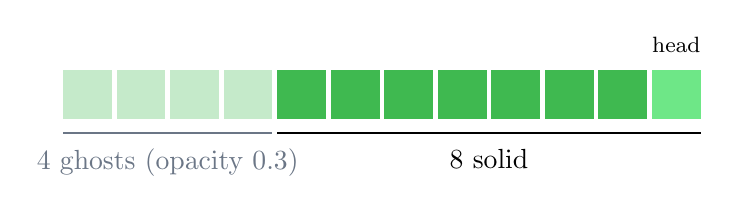
\begin{tikzpicture}[x=1cm,y=1cm]
  \def\seg{0.62}\def\pitch{0.68}
  \foreach \i in {0,...,11} {
    \pgfmathsetmacro{\x}{-\pitch*\i}
    \ifnum\i=0
      \fill[head] (\x,0) rectangle ++(\seg,\seg);
    \else
      \ifnum\i<8
        \fill[body] (\x,0) rectangle ++(\seg,\seg);
      \else
        \fill[body,fill opacity=0.3] (\x,0) rectangle ++(\seg,\seg);
      \fi
    \fi
  }
  % brackets and labels (head is segment 0 at the right)
  \draw[thick] (-\pitch*7,-0.18) -- (\seg,-0.18) node[midway,below=2pt] {8 solid};
  \draw[thick,ghostlabel] (-\pitch*11,-0.18) -- (-\pitch*8+\seg,-0.18)
    node[midway,below=2pt,text=ghostlabel] {4 ghosts (opacity 0.3)};
  \node[above=3pt,font=\footnotesize] at (\seg/2,\seg) {head};
\end{tikzpicture}
\caption{A snake of 12 segments: the head and the next 7 are solid, the 4 oldest are ghosts.
The size 8 is the constant \texttt{SOLID} in the game; the opacity 0.3 is the one it draws with.}
\end{figure}

\section*{How it was checked}
The 44 tests run the page's real script in a small JavaScript engine (QuickJS) with the browser parts replaced by stand-ins, and step the game by hand. They cover movement, walls, eating, the ghost boundary, pause and restart, and the score table.
\textbf{Not yet checked:} the game in a real browser (look, key handling, timing).

\section*{Rebuild this note}
\begin{verbatim}
cd note && pdflatex -interaction=nonstopmode snake-note.tex
uv run --no-project --with quickjs --with pytest pytest snake -q   # the tests
\end{verbatim}

\end{document}
